\documentclass[12pt,reqno]{article}
\usepackage{amsthm, amsmath, amsfonts, amssymb, amscd, mathtools, youngtab, euscript, mathrsfs, verbatim, enumerate, multicol, multirow, bbding, color, babel, esint, geometry, tikz, tikz-cd, tikz-3dplot, array, enumitem, hyperref, thm-restate, thmtools, datetime, graphicx, tensor, braket, slashed, standalone, pgfplots, ytableau, subfigure, wrapfig, dsfont, setspace, wasysym, pifont, float, rotating, adjustbox, pict2e,array}
\usepackage{amsmath}
\usepackage[utf8]{inputenc}
\usetikzlibrary{arrows, positioning, decorations.pathmorphing, decorations.pathreplacing, decorations.markings, matrix, patterns}
\tikzset{big arrow/.style={
    decoration={markings,mark=at position 1 with {\arrow[scale=1.5,#1]{>}}},
    postaction={decorate},
    shorten >=0.4pt},
  big arrow/.default=black}

\begin{document}

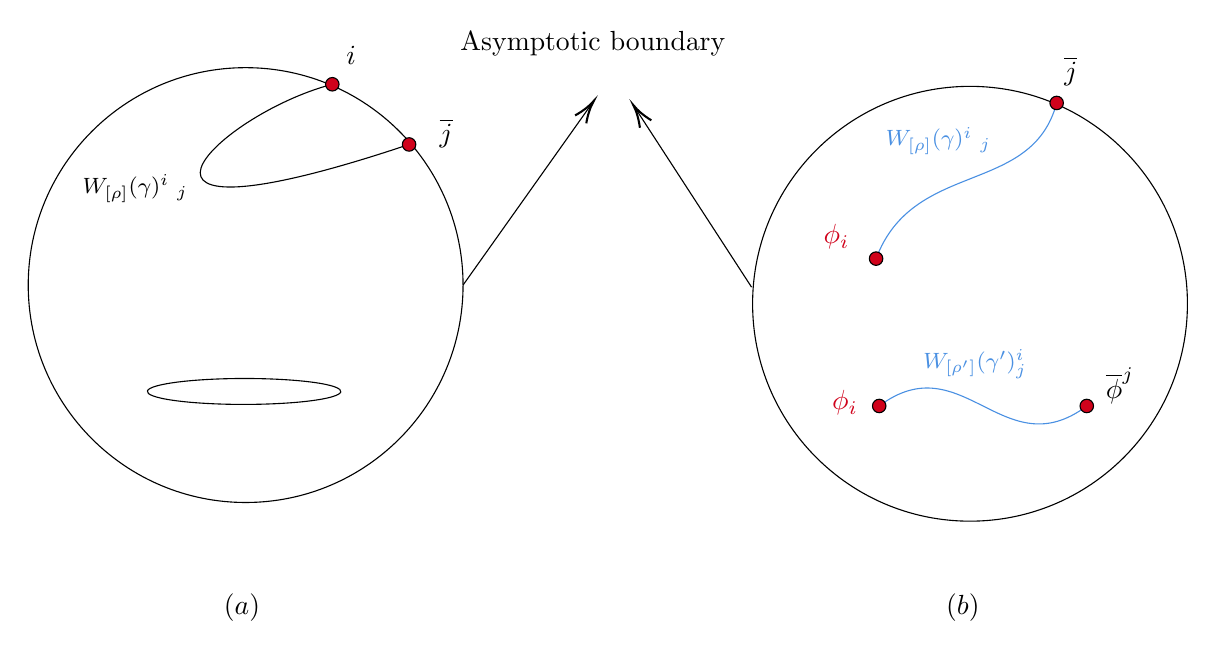
\begin{tikzpicture}[x=0.75pt,y=0.75pt,yscale=-1,xscale=1]

\draw [color={rgb, 255:red, 74; green, 144; blue, 226 }  ,draw opacity=1 ]   (455,198) .. controls (495,168) and (515,228) .. (555,198) ;
\draw [color={rgb, 255:red, 74; green, 144; blue, 226 }  ,draw opacity=1 ]   (453.5,127) .. controls (471.5,79) and (528.5,97) .. (540.5,52) ;
\draw   (45,139.75) .. controls (45,81.9) and (91.9,35) .. (149.75,35) .. controls (207.6,35) and (254.5,81.9) .. (254.5,139.75) .. controls (254.5,197.6) and (207.6,244.5) .. (149.75,244.5) .. controls (91.9,244.5) and (45,197.6) .. (45,139.75) -- cycle ;
\draw    (228.5,72) .. controls (67.5,126) and (134.5,58) .. (191.5,43) ;
\draw  [fill={rgb, 255:red, 208; green, 2; blue, 27 }  ,fill opacity=1 ] (188.25,43) .. controls (188.25,41.21) and (189.71,39.75) .. (191.5,39.75) .. controls (193.29,39.75) and (194.75,41.21) .. (194.75,43) .. controls (194.75,44.79) and (193.29,46.25) .. (191.5,46.25) .. controls (189.71,46.25) and (188.25,44.79) .. (188.25,43) -- cycle ;
\draw  [fill={rgb, 255:red, 208; green, 2; blue, 27 }  ,fill opacity=1 ] (225.25,72) .. controls (225.25,70.21) and (226.71,68.75) .. (228.5,68.75) .. controls (230.29,68.75) and (231.75,70.21) .. (231.75,72) .. controls (231.75,73.79) and (230.29,75.25) .. (228.5,75.25) .. controls (226.71,75.25) and (225.25,73.79) .. (225.25,72) -- cycle ;
\draw   (132.9,185.15) .. controls (157.07,183.94) and (183.87,185.58) .. (192.76,188.81) .. controls (201.65,192.05) and (189.27,195.64) .. (165.1,196.85) .. controls (140.93,198.06) and (114.13,196.42) .. (105.24,193.19) .. controls (96.35,189.95) and (108.73,186.36) .. (132.9,185.15) -- cycle ;
\draw   (394,148.75) .. controls (394,90.9) and (440.9,44) .. (498.75,44) .. controls (556.6,44) and (603.5,90.9) .. (603.5,148.75) .. controls (603.5,206.6) and (556.6,253.5) .. (498.75,253.5) .. controls (440.9,253.5) and (394,206.6) .. (394,148.75) -- cycle ;
\draw  [fill={rgb, 255:red, 208; green, 2; blue, 27 }  ,fill opacity=1 ] (537.25,52) .. controls (537.25,50.21) and (538.71,48.75) .. (540.5,48.75) .. controls (542.29,48.75) and (543.75,50.21) .. (543.75,52) .. controls (543.75,53.79) and (542.29,55.25) .. (540.5,55.25) .. controls (538.71,55.25) and (537.25,53.79) .. (537.25,52) -- cycle ;
\draw  [fill={rgb, 255:red, 208; green, 2; blue, 27 }  ,fill opacity=1 ] (450.25,127) .. controls (450.25,125.21) and (451.71,123.75) .. (453.5,123.75) .. controls (455.29,123.75) and (456.75,125.21) .. (456.75,127) .. controls (456.75,128.79) and (455.29,130.25) .. (453.5,130.25) .. controls (451.71,130.25) and (450.25,128.79) .. (450.25,127) -- cycle ;
\draw  [fill={rgb, 255:red, 208; green, 2; blue, 27 }  ,fill opacity=1 ] (451.75,198) .. controls (451.75,196.21) and (453.21,194.75) .. (455,194.75) .. controls (456.79,194.75) and (458.25,196.21) .. (458.25,198) .. controls (458.25,199.79) and (456.79,201.25) .. (455,201.25) .. controls (453.21,201.25) and (451.75,199.79) .. (451.75,198) -- cycle ;
\draw  [fill={rgb, 255:red, 208; green, 2; blue, 27 }  ,fill opacity=1 ] (551.75,198) .. controls (551.75,196.21) and (553.21,194.75) .. (555,194.75) .. controls (556.79,194.75) and (558.25,196.21) .. (558.25,198) .. controls (558.25,199.79) and (556.79,201.25) .. (555,201.25) .. controls (553.21,201.25) and (551.75,199.79) .. (551.75,198) -- cycle ;
\draw    (254.5,139.75) -- (316.34,52.63) ;
\draw [shift={(317.5,51)}, rotate = 125.37] [color={rgb, 255:red, 0; green, 0; blue, 0 }  ][line width=0.75]    (10.93,-3.29) .. controls (6.95,-1.4) and (3.31,-0.3) .. (0,0) .. controls (3.31,0.3) and (6.95,1.4) .. (10.93,3.29)   ;
\draw    (393.5,140.75) -- (337.59,54.68) ;
\draw [shift={(336.5,53)}, rotate = 56.99] [color={rgb, 255:red, 0; green, 0; blue, 0 }  ][line width=0.75]    (10.93,-3.29) .. controls (6.95,-1.4) and (3.31,-0.3) .. (0,0) .. controls (3.31,0.3) and (6.95,1.4) .. (10.93,3.29)   ;

% Text Node
\draw (252,16) node [anchor=north west][inner sep=0.75pt]   [align=left] {Asymptotic boundary};
% Text Node
\draw (70,85.4) node [anchor=north west][inner sep=0.75pt]  [font=\footnotesize]  {$W_{[ \rho ]}( \gamma )^{i} \ _{j}$};
% Text Node
\draw (197,23.4) node [anchor=north west][inner sep=0.75pt]    {$i$};
% Text Node
\draw (242,58.4) node [anchor=north west][inner sep=0.75pt]    {$\overline{j}$};
% Text Node
\draw (475,169.4) node [anchor=north west][inner sep=0.75pt]  [font=\footnotesize,color={rgb, 255:red, 74; green, 144; blue, 226 }  ,opacity=1 ]  {$W_{[ \rho ']}( \gamma ')_{j}^{i}$};
% Text Node
\draw (138,287.4) node [anchor=north west][inner sep=0.75pt]    {$( a)$};
% Text Node
\draw (486,287.4) node [anchor=north west][inner sep=0.75pt]    {$( b)$};
% Text Node
\draw (431,189.4) node [anchor=north west][inner sep=0.75pt]  [color={rgb, 255:red, 208; green, 2; blue, 27 }  ,opacity=1 ]  {$\phi _{i}$};
% Text Node
\draw (563,178.4) node [anchor=north west][inner sep=0.75pt]    {$\overline{\phi }^{j}$};
% Text Node
\draw (457,62.4) node [anchor=north west][inner sep=0.75pt]  [font=\footnotesize,color={rgb, 255:red, 74; green, 144; blue, 226 }  ,opacity=1 ]  {$W_{[ \rho ]}( \gamma )^{i} \ _{j}$};
% Text Node
\draw (543,28.4) node [anchor=north west][inner sep=0.75pt]    {$\overline{j}$};
% Text Node
\draw (427,109.4) node [anchor=north west][inner sep=0.75pt]  [color={rgb, 255:red, 208; green, 2; blue, 27 }  ,opacity=1 ]  {$\phi _{i}$};


\end{tikzpicture}

\end{document}